\documentclass[a4paper, 12pt]{article}
\usepackage[utf8]{inputenc}
\usepackage{hyperref}
\usepackage{geometry}
\usepackage{graphicx}
\geometry{margin=1in}
\title{Dokumentacja Projektu: \\ Automatyzacja Oceny Sprawozdań Studenckich przy Użyciu Dużych Modeli Językowych (StudentReportLLMs)}
\vspace{3cm}
\author{
    Magdalena Pakuła \and
    Jakub Pawlak \and
    Piotr Hynasiński \and
    Artur Pietrzak \and
    Rafał Górniak
}
\vspace{3cm}
\date{\today}

\begin{document}

\maketitle

\newpage
\tableofcontents
\newpage

\section{Wstęp}
\subsection{Cel dokumentu}
Celem niniejszego dokumentu jest przedstawienie szczegółowej dokumentacji projektowej dla systemu Automatyzacja Oceny Sprawozdań Studenckich przy Użyciu Dużych Modeli Językowych (StudentReportLLMs).
Dokument ma na celu opisanie zakresu projektu, jego celów, oraz definicji związanych z projektem.
Jest on przeznaczony dla wszystkich interesariuszy, w tym członków zespołu projektowego, kadry dydaktycznej oraz potencjalnych użytkowników systemu.

\subsection{Zakres projektu}
Projekt StudentReportLLMs obejmuje zaprojektowanie i implementację systemu wykorzystującego zaawansowane modele językowe do automatycznej oceny sprawozdań studenckich.
Ocena ma dotyczyć dwóch kluczowych aspektów: jakości treści oraz zgodności z wytycznymi projektowymi (konkretnego zadania, którego dotyczy sprawozdanie).
System ma również oceniać oryginalność tekstu w celu zapobiegania plagiatom.
Zakres prac obejmuje:

\begin{itemize}
    \item Analizę i projektowanie systemu, w tym zdefiniowanie głównych funkcji oraz wymagań technicznych.
    \item Wybór odpowiednich technologii i modeli językowych.
    \item Implementację systemu, w tym rozwój interfejsu użytkownika oraz integrację modeli językowych.
    \item Testowanie i ewaluację systemu.
\end{itemize}

\section{Terminy i definicje}

\begin{center}
\footnotesize
\begin{tabular}{|p{0.3\textwidth}|p{0.65\textwidth}|}
\hline
\textbf{Termin} & \textbf{Definicja} \\
\hline
LLMs (Large Language Models) & Zaawansowane modele językowe, takie jak GPT-4, BERT, T5, wykorzystywane do analizy i generowania tekstu. \\
\hline
Ocena jakości treści & Proces analizy sprawozdań pod kątem poprawności językowej, spójności oraz klarowności przekazywanych informacji. \\
\hline
Ocena zgodności z wytycznymi & Proces sprawdzania, czy sprawozdanie spełnia określone wymagania projektowe. \\
\hline
Plagiat & Nieuprawnione wykorzystanie cudzej pracy bez odpowiedniego uznania źródła, co projekt ma na celu wykrywać i zapobiegać. \\
\hline
Interfejs użytkownika (UI) & Platforma webowa umożliwiająca interakcję z systemem przez studentów i nauczycieli. \\
\hline
Information Retrieval & Proces wyszukiwania informacji w dużych zbiorach danych, który w projekcie będzie wspierany przez bazy danych i technologie zarządzania wektorami. \\
\hline
Duże modele językowe (LLMs) & Duże modele językowe to zaawansowane systemy sztucznej inteligencji, które zostały wytrenowane na ogromnych zbiorach danych tekstowych. LLMs są w stanie rozumieć i generować ludzką mowę w sposób, który imituje ludzkie pisanie. \\
\hline
Automatyzacja & Automatyzacja odnosi się do procesu zastępowania lub uzupełniania zadań wykonywanych przez ludzi zadaniami wykonywanymi przez maszyny lub programy komputerowe. Celem automatyzacji jest zwiększenie wydajności, obniżenie kosztów i minimalizacja błędów poprzez eliminację ludzkiego udziału lub zautomatyzowanie powtarzalnych zadań. \\
\hline
Tokenizacja & Proces podziału tekstu na mniejsze jednostki, zwane tokenami, co jest często używane w przetwarzaniu języka naturalnego, aby lepiej zrozumieć i analizować zawartość tekstu. \\
\hline
OCR (Optical Character Recognition) & Technologia pozwalająca na konwersję obrazów lub zeskanowanych dokumentów na edytowalny tekst, co jest istotne dla odczytu i analizy zawartości plików PDF. \\
\hline
Skalowalność systemu & Skalowalność systemu odnosi się do zdolności systemu do efektywnego dostosowywania się do wzrostu obciążenia lub zasobów. System jest uznawany za skalowalny, jeśli może rosnąć lub kurczyć się w zależności od potrzeb, zachowując przy tym swoją wydajność, niezawodność i funkcjonalność. \\
\hline
API (Application Programming Interface) & Interfejs programowania aplikacji, który umożliwia komunikację między różnymi komponentami oprogramowania, na przykład między systemem automatyzacji oceny a silnikami modeli językowych. \\
\hline
System odczytu i analizy plików & System zdolny do przetwarzania plików w formatach PDF, Word, LaTeX w celu analizy ich treści przez modele językowe. \\
\hline
\end{tabular}
\end{center}

\subsection{Opis potrzeby}
Głównym założeniem, a zarazem potrzebą jest wiarygodne, dokładne oraz z jak najmniejszym błędem sprawdzanie prac naukowych napisanych przez usługobiorców akademii, czyli studentów przy pomocy określonego narzędzia. Przy danych z góry kryteriach, program ma zachowywać się w należyty sposób.  Potrzeba zaistniała ze względu na możliwą stronniczość wykładowcy. Oznacza to, że osoby, które chodziły na wykłady, krewni bądź znajomi, osoby faworyzowane przez różne względy mogłyby być oceniane wyżej w porównaniu do reszty, za taką samą pracę. Następnym możliwym zagrożeniem jest błąd ludzki. W danej chwili, przy braku stu-procentowej pewności osoba sprawdzająca może niesłusznie odjąć punkty, podczas gdy rozwiązania, fraza zaproponowana przez studenta jest zupełnie poprawna i vice versa. Następną coraz większą “plagą” jest plagiat oraz paragrafy generowane przez sztuczną inteligencję. To również powinno być rozróżnione oraz wyłapane. Dlatego więc, aby każdy uczeń był równy wobec systemu sprawdzania, potrzebna jest technika, program to zapewniający. Ponadto każde konto uczelniane powinno mieć dostęp do tego rozwiązania, a zatem potrzebna jest autentykacja użytkownika dla studenta oraz nauczyciela, jako pośredniego administratora narzędzia.

\subsection{Zidentyfikowani osbiorcy}

\begin{center}
\footnotesize
\begin{tabular}{|p{0.2\textwidth}|p{0.7\textwidth}|}
\hline
\textbf{Nazwa} & \textbf{Opis} \\
\hline
Wykładowca (Nauczyciel akademicki) & Osoba pracująca w systemie oświaty w sektorze publicznym lub prywatnym w zależności od rodzaju miejsca pracy. Jednym z obowiązków zadawanie, a w konsekwencji sprawdzanie prac pisemnych, napisanych przez klientów uczelni lub kadry akademickiej w roli recenzenta. \\
\hline
Student (Uczeń) & Osoba realizująca ofertę uczelni, na której się znajduje w charakterze usługobiorcy. Pisze zadany przez nauczyciela raport, a następnie według kryteriów oceniania dostaje należytą informację zwrotną w postaci oceny. \\
\hline
\end{tabular}
\end{center}

\section{Opis systemu}
Projekt \textit{StudentRaportLLMs} polega na stworzeniu kompleksowego systemu opartego na zaawansowanych modelach językowych, który automatycznie oceni sprawozdania studenckie. System będzie przetwarzał tekst sprawozdań, analizując treść i sprawdzając zgodność z wytycznymi projektowymi lub innymi kryteriami. Na podstawie analizy, system będzie przyznawał oceny, dostosowane do konkretnego zadania lub przedmiotu. Aby zapewnić wiarygodność ocen, wyniki automatycznej oceny będą porównywane z wynikami ręcznie ocenionych sprawozdań, co pozwoli na dostosowanie parametrów oceniania i udoskonalenie procesu. Ponadto, system będzie integrowany z istniejącymi platformami edukacyjnymi, ułatwiając przesyłanie prac i wymianę informacji między studentami a nauczycielami. Projekt będzie elastyczny i przystosowany do zmian w technologiach oraz przepisach prawnych dotyczących ochrony danych osobowych.
\subsection{Zakres funkcjonalny}

System ma wykorzystywać duże modele językowe do oceny sprawozdań studenckich.
Ocena ma dotyczyć dwóch kluczowych aspektów: jakości treści i zgodności z wytycznymi projektowymi (konkretnego zadania,
którego dotyczy sprawozdanie).
Dzięki temu możliwe będzie szybkie, obiektywne i dokładne ocenianie treści sprawozdań oraz ich zgodności z wytycznymi projektowymi.
To rozwiązanie ma potencjał zrewolucjonizować proces oceniania, poprawiając jakość edukacji poprzez wprowadzenie bardziej obiektywnych i zgodnych z wytycznymi ocen.
Wymagane będzie zintegrowanie i wykorzystanie zaawansowanych modeli językowych, bez konieczności ich dodatkowego
szkolenia (fine-tuning).
Projekt powinien obejmować funkcjonalność odczytu i analizy plików w formatach PDF, Word, LaTeX. Dodatkowo, system musi
umożliwiać definiowanie przez operatora specyficznych kryteriów oceny, adaptowalnych do różnorodnych wymagań
projektowych.
Projekt zakłada również opracowanie metody oceny oryginalności tekstu, aby zapobiegać plagiatom i promować unikalność
prac studenckich.

\subsection{Zakres niefunkcjonalny}
Ważnym elementem będzie stworzenie intuicyjnego interfejsu użytkownika, który pozwoli na łatwe formułowanie zapytań
dotyczących specyficznych kryteriów oceny dla ogółu dostępnych prac, takich jak często popełniane błędy czy powtarzające
się braki w sprawozdaniach.
Kluczowymi elementami będą efektywność, precyzja oraz użyteczność systemu.
Ważne będzie również stworzenie szczegółowej dokumentacji projektowej.

\section{Wymagania}
Poniżej znajdują się wszystkie wymagania funkcjonalne i niefunkcjonalne projektu:

\subsection{Wymagania funkcjonalne}

\begin{enumerate}
    \item Zarządzanie kontami użytkowników
    \begin{enumerate}
        \item Tworzenie nowych kont
        \item Modyfikacja przywilejów istniejących kont
    \end{enumerate}
    \item Formułowanie przez nauczyciela kryteriów oceny pracy
    \item Analiza jakościowa treści sprawozdania
    \item Analiza zgodności z wymaganiami treści sprawozdania
    \item Porównanie pod kątem plagiatu z historycznymi pracami zapisanymi w uczelnianym archiwum
    \item Odczyt różnych formatów plików (.docx, .pdf, .tex)
    \item Zabezpieczenie przed atakami typu \textit{prompt injection}
\end{enumerate}

\subsection{Wymagania niefunkcjonalne}

\begin{enumerate}
    \item Intuicyjność i reaktywność interfejsu użytkownika
    \item Wysokie wartości miar porównujących wyniki automatycznego oraz manualnego sprawdzania:
    \begin{enumerate}
        \item F1-score
        \item Precision
        \item Recall
        \item Accuracy
    \end{enumerate}
    \item Pozytywna korelacja pomiędzy wynikami automatycznego i manualnego sprawdzania
    \item Automatyczne testy poprawności działania systemu
    \item Szczegółowa dokumentacja projektowa
    \item Satysfakcjonujący czas weryfikacji pracy przez system
\end{enumerate}

\subsection{Diagram przepływu danych}
DFD są szczególnie przydatne do przedstawienia przepływu danych i procesów w ramach systemu.
Poniżej na fig.~\ref{fig:dfd} znajduje się diagram przedstawiający, jak przetwarzane są dane w systemie.

\begin{figure}[H]
    \centering
    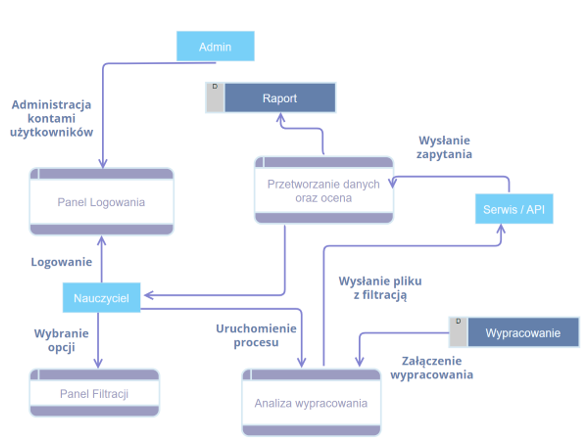
\includegraphics[width=\textwidth]{img/DFD}
    \caption{Diagram przepływu danych w systemie \textit{StudentReportLLMs}}
    \label{fig:dfd}
\end{figure}

\subsection{Diagram Business Process Model and Notation}
BPMN idealnie nadaje się do modelowania procesów biznesowych.
Poniżej na fig.~\ref{fig:BPMN} znajduje się diagram, który wskaże kluczowe procesy biznesowe związane z funkcjonalnością systemu.

\begin{figure}[H]
    \centering
    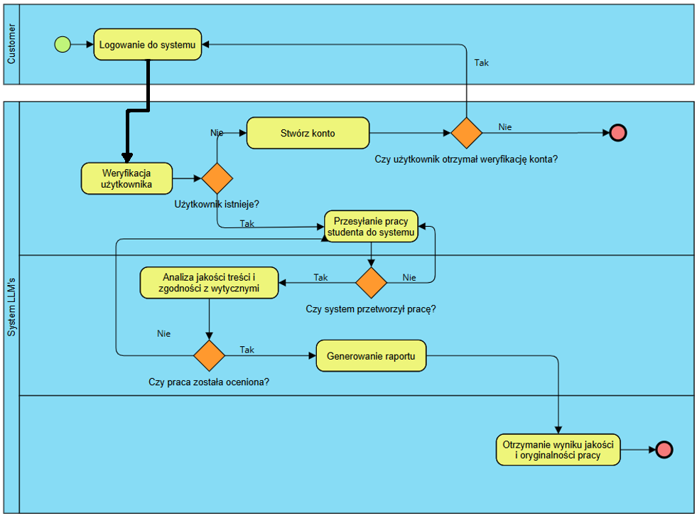
\includegraphics[width=\textwidth]{img/BPMN}
    \caption{Diagram Business Process Model and Notation systemu \textit{StudentReportLLMs}}
    \label{fig:BPMN}
\end{figure}

\subsection{Diagram SWOT}
Diagram SWOT (Strengths, Weaknesses, Opportunities, Threats) pokazany niżej na fig.~\ref{fig:swot} pomoże zidentyfikować wewnętrzne mocne strony, słabości oraz zewnętrzne szanse i zagrożenia.

\begin{figure}[H]
    \centering
    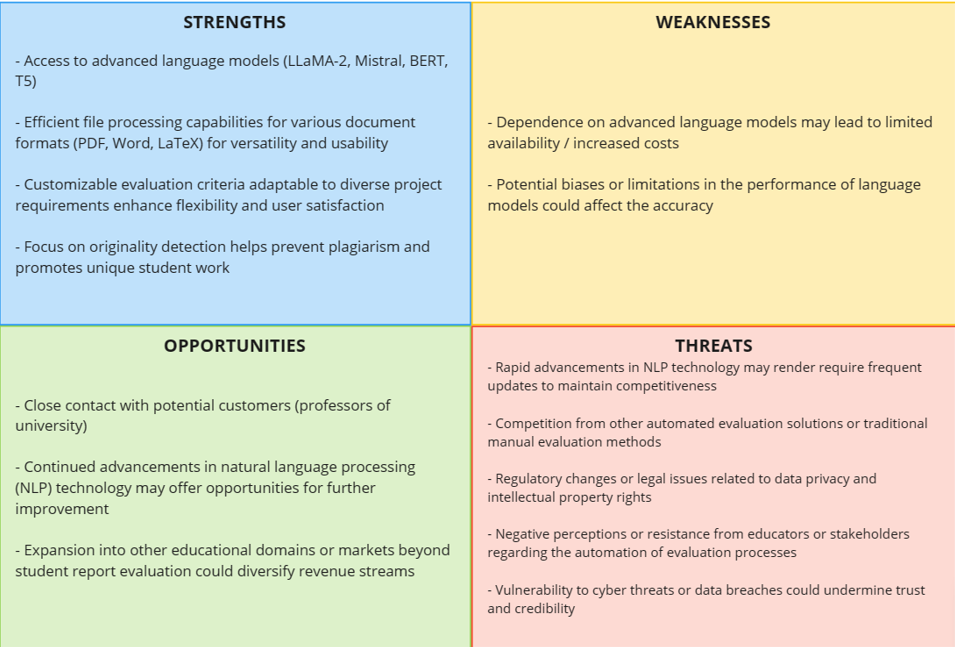
\includegraphics[width=\textwidth]{img/swot}
    \caption{Diagram SWOT systemu \textit{StudentReportLLMs}}
    \label{fig:swot}
\end{figure}

\subsection{Opis przypadków użycia}

\subsubsection{Przypadek użycia 1: Przesyłanie raportu do systemu}

\begin{table}[H]
\footnotesize
\centering
\caption{Przypadek użycia: Przesyłanie raportu do systemu}
\begin{tabular}{|p{0.45\linewidth}|p{0.45\linewidth}|}
\hline
\textbf{Typ} & Operacyjny \\
\hline
\textbf{Użytkownicy} & Nauczyciel akademicki \\
\hline
\textbf{Warunki wstępne} &
\begin{itemize}
    \item Nauczyciel musi być zalogowany do systemu.
    \item Raport studencki musi być w odpowiednim formacie (Word, PDF, LaTeX).
\end{itemize} \\
\hline
\textbf{Typowa kolejność kroków} &
\begin{enumerate}
    \item Nauczyciel loguje się do systemu "StudentReportLLMs".
    \item Nauczyciel wybiera opcję przesyłania nowego raportu.
    \item System wyświetla formularz do przesyłania pliku.
    \item Nauczyciel wypełnia formularz, dodając odpowiedni plik raportu oraz wszelkie dodatkowe informacje wymagane przez system (np. kategoria, autor, przedmiot).
    \item Nauczyciel przesyła formularz, a system zapisuje raport do bazy danych i wyświetla potwierdzenie poprawnego przesłania.
\end{enumerate} \\
\hline
\textbf{Warunki końcowe} &
\begin{itemize}
    \item Raport jest zapisany w systemie i oczekuje na automatyczną ocenę.
    \item Nauczyciel otrzymuje powiadomienie o poprawnym przesłaniu raportu.
\end{itemize} \\
\hline
\textbf{Alternatywna kolejność kroków} &
\begin{enumerate}
    \item Nauczyciel loguje się do systemu "StudentReportLLMs".
    \item Nauczyciel wybiera opcję przesyłania nowego raportu.
    \item System wyświetla formularz do przesyłania pliku.
    \item Nauczyciel próbuje przesłać plik w nieprawidłowym formacie.
    \item System wyświetla komunikat o błędzie i prosi o poprawienie formatu pliku.
    \item Nauczyciel poprawia format pliku i ponownie przesyła formularz.
    \item System zapisuje raport do bazy danych i wyświetla potwierdzenie poprawnego przesłania.
\end{enumerate} \\
\hline
\textbf{Komentarze i uwagi} &
\begin{itemize}
    \item System powinien obsługiwać różne formaty plików i weryfikować ich poprawność przed przesłaniem.
    \item System powinien być intuicyjny i łatwy w użyciu, aby nauczyciele mogli szybko i bezproblemowo przesyłać raporty.
\end{itemize} \\
\hline
\end{tabular}
\end{table}

\subsubsection{Przypadek użycia 2: Automatyczna ocena treści raportów}

\begin{table}[H]
\footnotesize
\centering
\caption{Przypadek użycia: Automatyczna ocena treści raportów}
\begin{tabular}{|p{0.45\linewidth}|p{0.45\linewidth}|}
\hline
\textbf{Typ} & Operacyjny \\
\hline
\textbf{Użytkownicy} & Nauczyciel akademicki \\
\hline
\textbf{Warunki wstępne} & 
\begin{itemize}
    \item Nauczyciel musi być zalogowany do systemu.
    \item Raport studencki musi być w odpowiednim formacie (Word, PDF, LaTeX).
    \item System musi mieć zdefiniowane kryteria oceny.
\end{itemize} \\
\hline
\textbf{Typowa kolejność kroków} &
\begin{enumerate}
    \item System wykrywa nowy przesłany raport oczekujący na ocenę.
    \item System analizuje treść raportu przy użyciu zaawansowanych modeli językowych.
    \item System sprawdza zgodność treści raportu z wytycznymi projektowymi i zdefiniowanymi kryteriami oceny.
    \item System generuje ocenę raportu oraz szczegółowy feedback dotyczący mocnych i słabych stron pracy.
    \item System zapisuje ocenę i feedback w bazie danych oraz powiadamia nauczyciela o zakończonej ocenie.
\end{enumerate} \\
\hline
\textbf{Warunki końcowe} & 
\begin{itemize}
    \item Nauczyciel musi być zalogowany do systemu.
    \item Raport zostaje oceniony i zapisany w systemie.
    \item Nauczyciel otrzymuje powiadomienie o zakończonej ocenie raportu.
\end{itemize} \\
\hline
\textbf{Alternatywna kolejność kroków} &
\begin{enumerate}
    \item System wykrywa nowy przesłany raport oczekujący na ocenę.
    \item System analizuje treść raportu przy użyciu zaawansowanych modeli językowych.
    \item System napotyka problem z analizą (np. nieczytelny tekst, błędy w formacie).
    \item System powiadamia nauczyciela o problemie i prosi o weryfikację raportu.
    \item Nauczyciel weryfikuje i poprawia raport, a następnie ponownie przesyła do systemu.
    \item System ponownie analizuje treść raportu, sprawdza zgodność z wytycznymi i generuje ocenę oraz feedback.
\end{enumerate} \\
\hline
\textbf{Komentarze i uwagi} &
\begin{itemize}
    \item System powinien być w stanie obsługiwać różne problemy z analizą i odpowiednio informować użytkownika o napotkanych błędach.
    \item System powinien zapewniać wysoką dokładność i spójność ocen, aby użytkownicy mogli ufać wynikowym ocenom.
\end{itemize} \\
\hline
\end{tabular}
\end{table}

\subsubsection{Przypadek użycia 3: Odczyt i konwersja plików}

\begin{table}[H]
\footnotesize
\centering
\caption{Przypadek użycia: Odczyt i konwersja plików}
\begin{tabular}{|p{0.45\linewidth}|p{0.45\linewidth}|}
\hline
\textbf{Typ} & Operacyjny \\
\hline
\textbf{Użytkownicy} & Nauczyciel akademicki \\
\hline
\textbf{Warunki wstępne} & 
\begin{itemize}
    \item Nauczyciel musi być zalogowany do systemu.
    \item Plik raportu musi być przesłany do systemu.
    \item System musi obsługiwać format pliku (Word, PDF, LaTeX).
\end{itemize} \\
\hline
\textbf{Typowa kolejność kroków} &
\begin{enumerate}
    \item Nauczyciel przesyła raport do systemu w jednym z obsługiwanych formatów (Word, PDF, LaTeX).
    \item System rozpoznaje format pliku i przystępuje do jego odczytu.
    \item System przetwarza plik, konwertując jego zawartość na format zrozumiały dla modeli językowych.
    \item System przeprowadza analizę zawartości przetworzonego pliku, identyfikując istotne sekcje i elementy raportu.
    \item System zapisuje przetworzoną i skonwertowaną wersję pliku w bazie danych oraz informuje nauczyciela o zakończeniu procesu konwersji.
\end{enumerate} \\
\hline
\textbf{Warunki końcowe} & 
\begin{itemize}
    \item Plik raportu jest poprawnie odczytany i skonwertowany.
    \item System zapisuje skonwertowaną wersję pliku w bazie danych.
    \item Nauczyciel otrzymuje powiadomienie o zakończeniu procesu konwersji.
\end{itemize} \\
\hline
\textbf{Alternatywna kolejność kroków} &
\begin{enumerate}
    \item Nauczyciel przesyła raport do systemu w jednym z obsługiwanych formatów (Word, PDF, LaTeX).
    \item System rozpoznaje format pliku i przystępuje do jego odczytu.
    \item System napotyka problem z odczytem pliku (np. uszkodzony plik, nieczytelny format).
    \item System powiadamia nauczyciela o problemie i prosi o weryfikację pliku.
    \item Nauczyciel poprawia plik i ponownie przesyła do systemu.
    \item System ponownie przetwarza plik, konwertując jego zawartość na format zrozumiały dla modeli językowych.
\end{enumerate} \\
\hline
\textbf{Komentarze i uwagi} &
\begin{itemize}
    \item System powinien być w stanie rozpoznać i poprawnie przetwarzać różne formaty plików używane przez nauczycieli.
    \item System powinien informować użytkowników o wszelkich problemach napotkanych podczas odczytu i konwersji plików, umożliwiając szybkie rozwiązanie problemów.
\end{itemize} \\
\hline
\end{tabular}
\end{table}

\subsubsection{Przypadek użycia 4: Personalizacja kryteriów oceny}

\begin{table}[H]
\footnotesize
\centering
\caption{Przypadek użycia: Personalizacja kryteriów oceny}
\begin{tabular}{|p{0.45\linewidth}|p{0.45\linewidth}|}
\hline
\textbf{Typ} & Operacyjny \\
\hline
\textbf{Użytkownicy} & Nauczyciel akademicki \\
\hline
\textbf{Warunki wstępne} & 
\begin{itemize}
    \item Nauczyciel musi być zalogowany do systemu.
\end{itemize} \\
\hline
\textbf{Typowa kolejność kroków} &
\begin{enumerate}
    \item Nauczyciel loguje się do systemu "StudentReportLLMs".
    \item Przechodzi do sekcji ustawień ocen.
    \item Modyfikuje istniejące kryteria oceny lub dodaje nowe według własnych preferencji. Zapisuje wprowadzone zmiany.
    \item System automatycznie uwzględnia nowe kryteria podczas oceny kolejnych raportów studenckich.
\end{enumerate} \\
\hline
\textbf{Warunki końcowe} & 
\begin{itemize}
    \item Zmodyfikowane kryteria oceny są zapisane i uwzględniane podczas kolejnych ocen raportów studenckich.
    \item Nauczyciel może dostosować proces oceniania do swoich potrzeb lub wymagań projektowych.
\end{itemize} \\
\hline
\textbf{Alternatywna kolejność kroków} &
\begin{enumerate}
    \item Nauczyciel loguje się do systemu "StudentReportLLMs".
    \item Przechodzi do sekcji ustawień ocen.
    \item Nauczyciel próbuje dodać nowe kryteria oceny, ale napotyka problem z zapisaniem zmian.
    \item System wyświetla komunikat o błędzie i prosi nauczyciela o ponowne zapisanie ustawień.
    \item Nauczyciel ponownie próbuje zapisać zmiany, a system potwierdza poprawne zastosowanie nowych kryteriów oceny.
\end{enumerate} \\
\hline
\textbf{Komentarze i uwagi} &
\begin{itemize}
    \item Interfejs użytkownika systemu powinien być intuicyjny i łatwy w obsłudze, aby nauczyciel mógł bezproblemowo dostosować kryteria oceny.
    \item System powinien zapewnić odpowiednie komunikaty o błędach w przypadku problemów podczas zapisywania zmian w ustawieniach ocen.
    \item Warto umożliwić nauczycielowi podgląd zmian przed ich zatwierdzeniem, aby uniknąć niezamierzonych modyfikacji kryteriów oceny.
\end{itemize} \\
\hline
\end{tabular}
\end{table}

\subsubsection{Przypadek użycia 5: Ogólne korzystanie z sytemu przez użytkownika}
W tym przypadku przedstawiony będzie diagram przypadku użycia na figurze~\ref{fig:use-case-diagram}.

\begin{figure}[H]
    \centering
    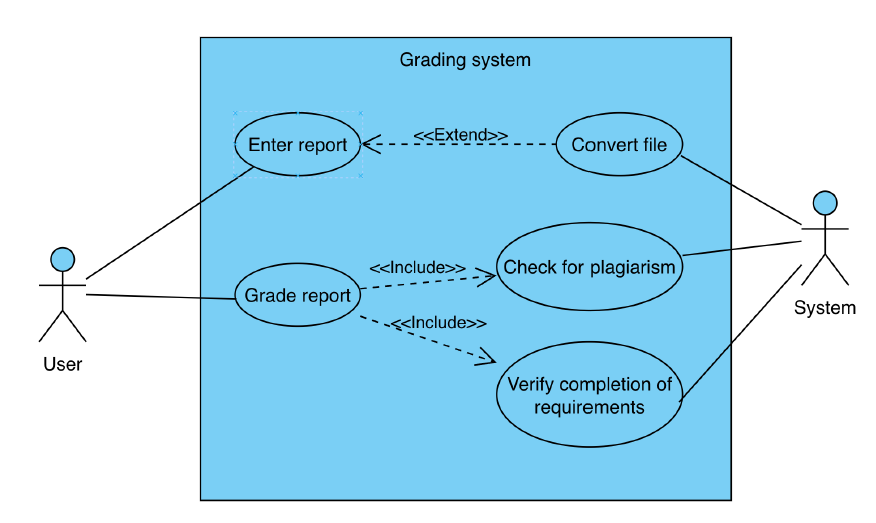
\includegraphics[width=\textwidth]{img/usecase_diagram}
    \caption{Diagram przypadku użycia \textit{StudentReportLLMs}}
    \label{fig:use-case-diagram}
\end{figure}

\section{Architektura Systemu}
W tej sekcji przedstawiono architekturę systemu \textit{StudentReportLLMs}, który ma na celu automatyzację oceny sprawozdań studenckich przy użyciu dużych modeli językowych.

\subsection{Architektura ogólna}

Architektura systemu oparta jest na mikroserwisach, co umożliwia łatwą skalowalność i niezależność poszczególnych komponentów. Główne komponenty architektoniczne to:

\begin{itemize}
    \item \textbf{Frontend}: Interfejs użytkownika (UI), dostępny jako aplikacja webowa umożliwiająca studentom przesyłanie swoich sprawozdań oraz przeglądanie ocen.
    \item \textbf{Backend}: Centralny serwis zarządzający, który obsługuje logikę biznesową, integrację z modelami językowymi oraz zarządzanie zadaniami oceny.
    \item \textbf{Serwisy modeli językowych}: Oddzielne serwisy odpowiedzialne za integrację z różnymi modelami językowymi (np. GPT-4, BERT), które wykonują analizę i ocenę tekstu.
    \item \textbf{Baza danych}: Centralna baza danych przechowująca skonwertowane sprawozdania oraz baza dancyh do analizy i przetwarzania sprawozdań.
    \item \textbf{System odczytu i analizy plików}: Serwis do przetwarzania plików w formatach PDF, Word, LaTeX, konwertujący je na tekst, który jest następnie przekazywany do serwisów modeli językowych.
\end{itemize}

Architektura opiera się na komunikacji asynchronicznej oraz zastosowaniu API do integracji poszczególnych komponentów.

\subsection{Diagram komponentów}

Poniżej, na figurze~\ref{fig:architecture}, przedstawiono diagram komponentów architektonicznych systemu \textit{StudentReportLLMs}, który ilustruje interakcje między poszczególnymi serwisami:

\begin{figure}[H]
    \centering
    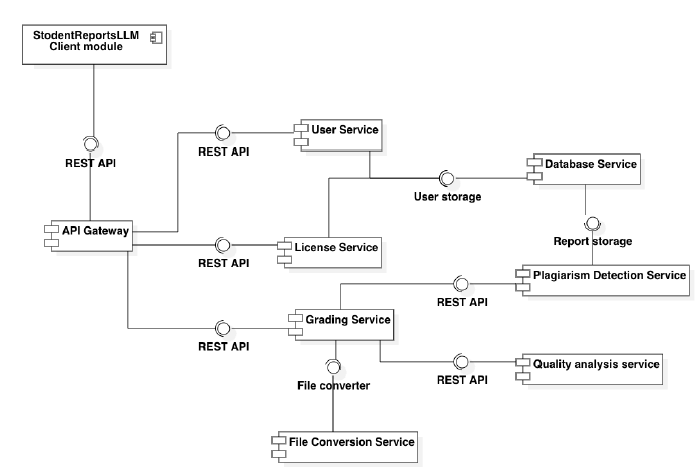
\includegraphics[width=\textwidth]{img/component_diagram}
    \caption{Diagram komponentów architektonicznych systemu \textit{StudentReportLLMs}}
    \label{fig:architecture}
\end{figure}

Diagram pokazuje strukturę systemu oraz przepływ danych między serwisami. Frontend komunikuje się z backendem poprzez API, a backend zarządza komunikacją z serwisami modeli językowych oraz bazą danych.

\subsection{Diagram klas}
Poniżej, na figurze~\ref{fig:class-diagram}, przedstawiono diagram klas systemu \textit{StudentReportLLMs}, który ilustruje klasy i ich relacje:
\begin{figure}[H]
    \centering
    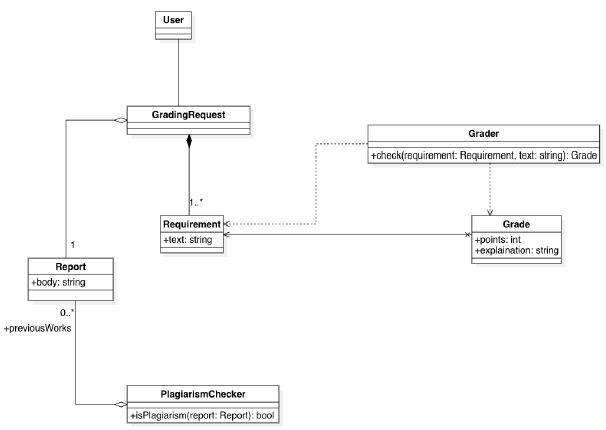
\includegraphics[width=\textwidth]{img/class_diagram}
    \caption{Diagram klas h systemu \textit{StudentReportLLMs}}
    \label{fig:class-diagram}
\end{figure}

\subsection{Technologie i narzędzia}

Do realizacji projektu \textit{StudentReportLLMs} wykorzystano szereg nowoczesnych technologii i narzędzi:

\begin{itemize}
    \item \textbf{Frontend}: React.js
    \item \textbf{Backend}: Node.js, Python (do integracji z modelami językowymi)
    \item \textbf{Baza danych}: MongoDB, QDRANT
    \item \textbf{Serwisy modeli językowych}: Python, TensorFlow, Hugging Face Transformers
    \item \textbf{System kontroli wersji}: Git, GitHub
    \item \textbf{Konteneryzacja}: Docker
    \item \textbf{Zarządzanie zadaniami}: RabbitMQ
\end{itemize}

\subsection{Bezpieczeństwo}

Bezpieczeństwo systemu \textit{StudentReportLLMs} zapewniono poprzez:

\begin{itemize}
    \item Uwierzytelnianie i autoryzację użytkowników przy użyciu JWT (JSON Web Token).
    \item Zabezpieczenia API przed atakami typu \textit{SQL injection} oraz \textit{cross-site scripting (XSS)}.
    \item Szyfrowanie danych przechowywanych w bazie danych oraz w transmisji między serwisami.
\end{itemize}

Podjęto także środki ostrożności, aby zapewnić zgodność z przepisami o ochronie danych osobowych (GDPR).

\section{Projekt Interfejsu}
Projekt interfejsu użytkownika (UI) systemu \textit{StudentReportLLMs} ma na celu zapewnienie intuicyjnej, efektywnej i przyjaznej dla użytkownika platformy, umożliwiającej łatwą interakcję studentów oraz nauczycieli z systemem automatycznej oceny sprawozdań studenckich. Interfejs powinien być dostosowany do potrzeb różnych użytkowników, zapewniając transparentność oceniania oraz dostęp do szczegółowych informacji na temat wyników i zaleceń.

\subsection{Założenia projektowe}

Główne założenia projektowe interfejsu użytkownika obejmują:

\begin{itemize}
\item Prostota obsługi: Interfejs powinien być intuicyjny i łatwy w nawigacji, co umożliwi szybkie i efektywne korzystanie zarówno studentom, jak i nauczycielom.
\item Responsywność: Interfejs powinien być responsywny, dostosowując się automatycznie do różnych urządzeń (komputery, tablety, telefony), co zapewni pełen dostęp do funkcjonalności systemu niezależnie od używanego urządzenia.
\item Personalizacja: System powinien umożliwiać personalizację doświadczenia użytkownika, na przykład poprzez dostosowanie preferencji wyświetlania danych lub ustawień powiadomień.
\item Bezpieczeństwo: Interfejs powinien zapewniać wysoki poziom bezpieczeństwa danych osobowych i wyników oceniania, zgodnie z obowiązującymi przepisami o ochronie danych.
\item Wizualizacja danych: System powinien oferować czytelne i przejrzyste prezentowanie wyników oceniania, statystyk oraz raportów, aby użytkownicy mogli łatwo analizować i interpretować zgromadzone dane.
\end{itemize}

\subsection{Elementy interfejsu}

Interfejs użytkownika systemu \textit{StudentReportLLMs} będzie zawierać następujące kluczowe elementy:

\begin{itemize}
\item Panel logowania: Dedykowany dla studentów i nauczycieli, umożliwiający autentykację i dostęp do odpowiednich funkcji systemu.
\item Panel administracyjny: Dla administratorów systemu, zapewniający zarządzanie użytkownikami, ustawieniami systemu oraz raportami.
\item Formularz wysyłania sprawozdań: Umożliwiający studentom przesyłanie swoich prac w różnych formatach (PDF, Word, LaTeX).
\item Wyświetlanie wyników: Interaktywne wyświetlanie wyników oceniania, z możliwością szczegółowego przeglądu komentarzy i zaleceń.
\item Panel konfiguracyjny kryteriów oceny: Dla nauczycieli, umożliwiający definiowanie specyficznych kryteriów oceniania dostosowanych do wymagań projektowych.
\item Powiadomienia: System powinien obsługiwać powiadomienia w czasie rzeczywistym, informujące o statusie ocen, komunikatach od nauczycieli oraz innych istotnych wydarzeniach.
\end{itemize}

Projekt interfejsu będzie stale ewoluował na podstawie feedbacku użytkowników oraz zmieniających się potrzeb edukacyjnych, zapewniając wysoką użyteczność i satysfakcję z jego użytkowania.

\section{Testowanie}
Testowanie systemu \textit{StudentReportLLMs} odgrywa kluczową rolę w zapewnieniu jego niezawodności, funkcjonalności oraz zgodności z wymaganiami. Proces testowania obejmuje szeroki zakres działań mających na celu sprawdzenie każdego aspektu systemu, zarówno pod kątem jego działania technicznego, jak i użyteczności.

\subsection{Cele testowania}

Główne cele testowania systemu \textit{StudentReportLLMs} obejmują:

\begin{itemize}
\item Weryfikacja poprawności funkcjonalnej: Testowanie ma na celu sprawdzenie, czy wszystkie funkcjonalności systemu działają zgodnie z założeniami i spełniają oczekiwania użytkowników.
\item Ocena wydajności: Testy wydajnościowe pomagają określić, jak system radzi sobie z różnym obciążeniem, zapewniając odpowiednią reaktywność i szybkość działania.
\item Bezpieczeństwo: Testowanie bezpieczeństwa ma na celu zidentyfikowanie potencjalnych luk oraz zagrożeń związanych z dostępem do danych osobowych i bezpieczeństwem systemu jako całości.
\item Testy integracyjne: Sprawdzają, czy poszczególne komponenty systemu współpracują ze sobą zgodnie z założeniami projektowymi, zapewniając pełną funkcjonalność.
\item Testy użyteczności: Ocena interfejsu użytkownika pod kątem intuicyjności, łatwości obsługi oraz zgodności z oczekiwaniami użytkowników końcowych.
\item Testy wydajności modeli językowych: Sprawdzenie, czy zastosowane duże modele językowe działają zgodnie z oczekiwaniami pod względem generacji tekstu, analizy treści i oceny oryginalności.
\end{itemize}

\subsection{Metodologia testowania}

Proces testowania systemu \textit{StudentReportLLMs} będzie oparty na zintegrowanych metodologiach testowych, obejmujących:

\begin{itemize}
\item Testy jednostkowe: Sprawdzenie poprawności działania poszczególnych komponentów systemu oraz ich izolowanych funkcji.
\item Testy integracyjne: Weryfikacja współpracy różnych komponentów systemu i ich interakcji, aby zapewnić spójność i pełną funkcjonalność systemu.
\item Testy akceptacyjne: Przeprowadzenie testów z udziałem użytkowników końcowych, aby ocenić, czy system spełnia ich oczekiwania oraz czy jest łatwy w użyciu.
\item Testy wydajnościowe: Ocena wydajności systemu pod względem czasu odpowiedzi, obciążenia i stabilności działania w różnych warunkach.
\item Testy bezpieczeństwa: Weryfikacja odporności systemu na ataki typu \textit{SQL injection}, \textit{cross-site scripting} oraz inne potencjalne zagrożenia.
\end{itemize}

\subsection{Plan testów}

Plan testów obejmuje szczegółowe scenariusze testowe dla każdej funkcjonalności systemu, uwzględniając różne przypadki użycia, typowe błędy użytkowników oraz nieoczekiwane sytuacje. Każdy test będzie dokumentowany, a wyniki będą analizowane i raportowane, co umożliwi identyfikację i szybkie rozwiązywanie napotkanych problemów.

\begin{enumerate}
\item \textbf{Sprawdzenie czasu przetwarzania sprawozdań studenckich przez model językowy}
   \begin{itemize}
   \item \textbf{Opis przypadku testowego:} Czas przetwarzania sprawozdań studenckich nie powinien przekraczać 15-20 sekund.
   \item \textbf{Kroki potrzebne do przeprowadzenia testu:}
     \begin{enumerate}
     \item Przesłanie sprawozdania studenckiego do systemu i oczekiwanie na przetworzenie.
     \item Rozpoczęcie przetwarzania sprawozdania studenckiego przez model językowy oraz rozpoczęcie odmierzania czasu.
     \item Weryfikacja czy czas przetwarzania jest akceptowalny.
     \end{enumerate}
   \item \textbf{Oczekiwane rezultaty:} System przetwarza sprawozdanie studenckie w akceptowalnym czasie.
   \end{itemize}

\item \textbf{Sprawdzenie czy system poprawnie analizuje jakość treści sprawozdania}
   \begin{itemize}
   \item \textbf{Opis przypadku testowego:} Jakość treści jest analizowana, a system generuje raport końcowy.
   \item \textbf{Kroki potrzebne do przeprowadzenia testu:}
     \begin{enumerate}
     \item Przesłanie sprawozdania studenckiego do analizy jakości treści.
     \item Uruchomienie funkcji analizy jakości treści.
     \item Sprawdzenie wygenerowanego raportu oceny jakości.
     \end{enumerate}
   \item \textbf{Oczekiwane rezultaty:} System prawidłowo analizuje jakość treści sprawozdania i generuje raport po zakończeniu procesu.
   \end{itemize}

\item \textbf{Sprawdzenie czy system poprawnie ocenia zgodność z wytycznymi projektowymi}
   \begin{itemize}
   \item \textbf{Opis przypadku testowego:} Zgodność sprawozdania z wytycznymi jest oceniana.
   \item \textbf{Kroki potrzebne do przeprowadzenia testu:}
     \begin{enumerate}
     \item Przesłanie sprawozdania studenckiego do oceny zgodności z wytycznymi.
     \item Zdefiniowanie specyficznych kryteriów oceny zgodnie z wytycznymi projektowymi.
     \item Uruchomienie funkcji oceny zgodności z wytycznymi.
     \item Sprawdzenie wyników działania funkcji względem wytycznych.
     \end{enumerate}
   \item \textbf{Oczekiwane rezultaty:} System prawidłowo ocenia zgodność sprawozdania z wytycznymi projektowymi.
   \end{itemize}

\item \textbf{Sprawdzenie funkcji oceny oryginalności tekstu}
   \begin{itemize}
   \item \textbf{Opis przypadku testowego:} Wykrywanie plagiatu.
   \item \textbf{Kroki potrzebne do przeprowadzenia testu:}
     \begin{enumerate}
     \item Przesłanie sprawozdania studenckiego podejrzanego o plagiat.
     \item Uruchomienie funkcji oceny oryginalności tekstu.
     \item Sprawdzenie raportu oryginalności.
     \end{enumerate}
   \item \textbf{Oczekiwane rezultaty:} System identyfikuje zduplikowane fragmenty i generuje wynik oceny oryginalności.
   \end{itemize}

\item \textbf{Sprawdzenie kompatybilności systemu z różnymi formatami plików}
   \begin{itemize}
   \item \textbf{Opis przypadku testowego:} Kompatybilność z formatami plików PDF, Word, LaTeX - rezultaty powinny być te same dla każdego formatu.
   \item \textbf{Kroki potrzebne do przeprowadzenia testu:}
     \begin{enumerate}
     \item Przesłanie sprawozdań studenckich w formatach PDF, Word i LaTeX.
     \item Uruchomienie funkcji analizy jakości i oceny zgodności dla każdego formatu pliku.
     \item Porównanie wyników dla każdego formatu.
     \end{enumerate}
   \item \textbf{Oczekiwane rezultaty:} System poprawnie odczytuje i przetwarza sprawozdania we wszystkich obsługiwanych formatach.
   \end{itemize}

    \item \textbf{Testowanie interfejsu użytkownika pod kątem łatwości użytkowania}
   \begin{itemize}
   \item \textbf{Opis przypadku testowego:} Intuicyjny interfejs użytkownika.
   \item \textbf{Kroki potrzebne do przeprowadzenia testu:}
     \begin{enumerate}
     \item Nawigacja po interfejsie użytkownika w celu uzyskania dostępu do różnych funkcji.
     \item Formułowanie zapytań oceny za pomocą dostępnego interfejsu.
     \end{enumerate}
   \item \textbf{Oczekiwane rezultaty:} Interfejs użytkownika jest intuicyjny i umożliwia łatwą interakcję z systemem.
   \end{itemize}

\item \textbf{Testowanie integracji systemu z modelami językowymi}
   \begin{itemize}
   \item \textbf{Opis przypadku testowego:} Integracja z modelami językowymi bez potrzeby dodatkowego szkolenia.
   \item \textbf{Kroki potrzebne do przeprowadzenia testu:}
     \begin{enumerate}
     \item Upewnienie się, że modele językowe są zintegrowane bez potrzeby dodatkowego szkolenia.
     \item Uruchomienie analizy jakości i oceny zgodności za pomocą tych modeli.
     \end{enumerate}
   \item \textbf{Oczekiwane rezultaty:} System skutecznie integruje i wykorzystuje modele językowe do analizy i oceny.
   \end{itemize}

\end{enumerate}

\subsection{Ewaluacja i raportowanie}

Po zakończeniu testów zostanie przeprowadzona ocena ich wyników oraz przygotowany raport z rekomendacjami dotyczącymi dalszych działań. Wszystkie ustalone nieprawidłowości będą korygowane, a system będzie testowany ponownie w celu potwierdzenia poprawności wprowadzonych zmian.
\section{Wdrożenie}
Proces wdrożenia systemu \textit{StudentReportLLMs} obejmuje szereg kluczowych działań mających na celu zapewnienie płynnego uruchomienia i użytkowania systemu przez jego użytkowników końcowych.

\subsection{Przygotowanie środowiska wdrożeniowego}

Pierwszym krokiem w procesie wdrożenia jest przygotowanie odpowiedniego środowiska do uruchomienia systemu. Będzie to obejmować:

\begin{itemize}
\item Instalacja i konfiguracja serwerów: Zapewnienie odpowiedniej infrastruktury serwerowej, która będzie obsługiwać aplikację oraz przechowywać dane.
\item Konfiguracja baz danych: Utworzenie i skonfigurowanie odpowiednich baz danych potrzebnych do przechowywania danych użytkowników, sprawozdań studenckich oraz wyników ocen.
\item Instalacja zewnętrznych zależności: Zapewnienie, że wszystkie zewnętrzne biblioteki, narzędzia i modele językowe, które są niezbędne do działania systemu, są poprawnie zainstalowane i skonfigurowane.
\end{itemize}

W celu przedstawienia procesu wdrożenia, poniższy rusynek na~\ref{fig:wdrozenie} przedstawia diagram wdrożenia.

\begin{figure}[H]
    \centering
    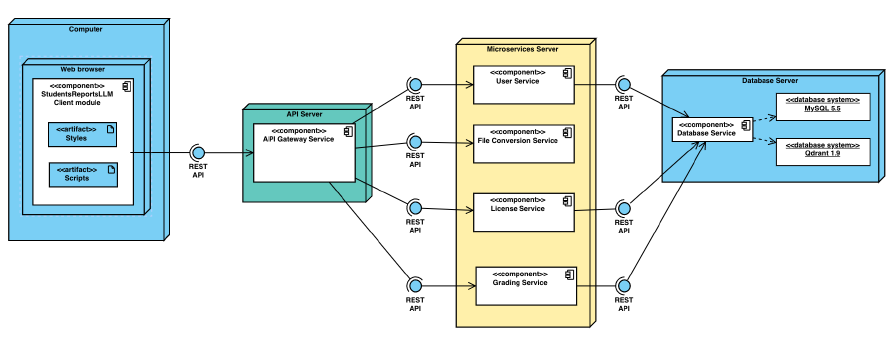
\includegraphics[width=\textwidth]{img/diagram_wdrozenia}
    \caption{Diagram wdrożenia systemu \textit{StudentReportLLMs}}
    \label{fig:wdrozenie}
\end{figure}

\subsection{Testowanie w środowisku produkcyjnym}

Przed przejściem do pełnego wdrożenia, system będzie poddany intensywnym testom w środowisku produkcyjnym. Celem jest upewnienie się, że wszystkie funkcjonalności działają zgodnie z oczekiwaniami oraz że system jest odporny na obciążenie i gotowy do użytku.

\subsection{Szkolenie użytkowników}

Kolejnym krokiem będzie przeprowadzenie szkoleń dla użytkowników końcowych systemu, w tym dla wykładowców i studentów. Szkolenia te mają na celu zapoznanie użytkowników z interfejsem systemu, jego funkcjonalnościami oraz procedurami postępowania, takimi jak przesyłanie sprawozdań, formułowanie kryteriów oceny oraz interpretacja wyników ocen.

\subsection{Pełne wdrożenie systemu}

Gdy wszystkie powyższe kroki zostaną zakończone pomyślnie, system \textit{StudentReportLLMs} zostanie w pełni wdrożony do użytku. Proces ten będzie monitorowany i wspierany przez zespół techniczny, który będzie gotowy reagować na ewentualne problemy i pytania użytkowników.

\subsection{Monitorowanie i utrzymanie}

Po wdrożeniu systemu będzie kontynuowane monitorowanie jego działania oraz regularne aktualizacje i utrzymywanie systemu. Celem jest zapewnienie wysokiej dostępności, bezpieczeństwa oraz efektywności działania systemu w dłuższym okresie.
\section{Utrzymanie i wsparcie}
Utrzymanie i wsparcie systemu \textit{StudentReportLLMs} jest kluczowe dla zapewnienia jego stabilności, bezpieczeństwa oraz efektywności w długim okresie użytkowania. Proces utrzymania i wsparcia obejmuje szereg działań mających na celu monitorowanie, utrzymanie oraz ewentualne rozwijanie systemu w odpowiedzi na potrzeby użytkowników.

\subsection{Monitorowanie systemu}

Podstawowym elementem utrzymania systemu jest ciągłe monitorowanie jego działania. Proces monitorowania powinien obejmować:

\begin{itemize}
\item Monitorowanie wydajności: Śledzenie wydajności systemu, w tym czasu odpowiedzi, zużycia zasobów oraz obciążenia serwera, aby zapewnić płynne działanie bez opóźnień.
\item Monitorowanie bezpieczeństwa: Analiza logów w celu wczesnego wykrywania potencjalnych zagrożeń bezpieczeństwa, takich jak próby nieautoryzowanego dostępu czy ataki typu DDoS.
\item Monitorowanie błędów: Zbieranie informacji o błędach systemowych oraz aplikacyjnych, aby szybko identyfikować i naprawiać ewentualne problemy.
\end{itemize}

\subsection{Wsparcie użytkowników}

System \textit{StudentReportLLMs} powinien zapewniać efektywne wsparcie dla swoich użytkowników, w tym dla wykładowców oraz studentów. Wsparcie użytkowników może obejmować:

\begin{itemize}
\item Pomoc techniczna: Udzielanie szybkiej odpowiedzi na pytania techniczne oraz rozwiązywanie problemów związanych z działaniem systemu.
\item Wsparcie użytkowe: Szkolenie użytkowników w zakresie korzystania z systemu, w tym omówienie procedur, interpretacji wyników ocen oraz wyjaśnienie funkcjonalności.
\item Obsługa zgłoszeń: Zapewnienie efektywnego procesu obsługi zgłoszeń użytkowników, w tym bieżącego informowania o postępie rozwiązania problemu.
\end{itemize}

\subsection{Aktualizacje i rozwój systemu}

Aby system \textit{StudentReportLLMs} pozostał aktualny i efektywny, konieczne jest regularne wprowadzanie aktualizacji oraz rozwijanie jego funkcjonalności. Proces ten powinien być oparty na:

\begin{itemize}
\item Analizie feedbacku: Analiza opinii użytkowników oraz ich sugestii dotyczących usprawnień i nowych funkcjonalności systemu.
\item Planowaniu aktualizacji: Określenie harmonogramu i zakresu kolejnych aktualizacji systemu, aby zapewnić minimalne zakłócenia w jego działaniu.
\item Rozwój funkcjonalności: Implementacja nowych funkcji oraz usprawnień zgodnie z wymaganiami użytkowników oraz rozwojem technologii.
\end{itemize}

\subsection{Zarządzanie dokumentacją}

Aby zapewnić przejrzystość i dostępność informacji, niezbędne jest prowadzenie aktualnej dokumentacji systemu, która zawiera opisy funkcjonalności, procedur obsługi, historię zmian oraz plany rozwoju.
\section{Zarządzanie projektem}
\subsection{Harmonogram}
\begin{center}
\footnotesize
\begin{tabular}{|p{0.3\textwidth}|c|c|c|c|}
\hline
\textbf{Name / Description} & \textbf{Priority} & \textbf{Size estimate (Points)} & \textbf{State} & \textbf{Target iteration} \\
\hline
Określenie celów oraz założeń & 5 & 1 & Zrobione & 1 \\
\hline
Określenie kosztów z uwzględnieniem amortyzacji oraz wstępnego planu realizacji & 4 & 2 & Zrobione & 1 \\
\hline
Wyznaczenie głównych funkcji dla członków drużyny projektowej & 5 & 1 & W trakcie & 1 \\
\hline
Określenie wymagań funkcjonalnych oraz niefunkcjonalnych & 5 & 2 & Nie zrobione & 1 \\
\hline
Zdefiniowanie środowiska oraz kluczowych komponentów & 4 & 3 & Nie zrobione & 1 \\
\hline
Podzielenie projektu na zadania & 4 & 4 & W trakcie & 1 \\
\hline
Utworzenie harmonogramu z pewną niepewnością czasową & 4 & 4 & Zrobione & 1 \\
\hline
Przydzielenie zadań dla developerów & 3 & 2 & Nie zrobione & 1 \\
\hline
Głęboka analiza rynku wraz ze sprawdzeniem podobnych już rozwiązań & 4 & 8 & Nie zrobione & 2 \\
\hline
Wyłuskanie wad i zalet z aplikacji & 3 & 3 & Nie zrobione & 2 \\
\hline
Poszukiwania odpowiednich modeli językowych & 5 & 5 & Nie zrobione & 2 \\
\hline
Znalezienie danych testowych dla modelu, sprawdzenia dokładności & 4 & 4 & Nie zrobione & 2 \\
\hline
Zbudowanie interfejsu użytkownika GUI & 5 & 16 & Nie zrobione & 2 \\
\hline
Zaprogramowanie interfejsu dla plików wejściowych różnego rozszerzenia & 4 & 16 & Nie zrobione & 2 \\
\hline
Dodanie funkcjonalności manipulacji opcją sprawdzenia & 4 & 16 & Nie zrobione & 2 \\
\hline
Zaprogramowanie modułu sprawdzającego (edycja modelu) & 5 & 32 & Nie zrobione & 2 \\
\hline
Testowanie oprogramowania & 4 & 16 & Nie zrobione & 2 \\
\hline
Sprawdzanie spełnionych założeń & 5 & 8 & Nie zrobione & 3 \\
\hline
Naprawienie potrzebnych niedociągnięć & 5 & 8 & Nie zrobione & 3 \\
\hline
Dostarczenie dokumentacji technicznej & 5 & 24 & Nie zrobione & 3 \\
\hline
\end{tabular}
\end{center}

\end{document}
